\documentclass[tikz,border=10pt]{standalone}
\usepackage[T1]{fontenc}
\usepackage{lmodern}
\usetikzlibrary{positioning, fit, backgrounds, arrows.meta, calc}

\definecolor{datalayerborder}{HTML}{70ad47}
\definecolor{datalayerfill}{HTML}{e2f0d9}
\definecolor{modelborder}{HTML}{d6b656}
\definecolor{modelfill}{HTML}{fff2cc}
\definecolor{kernelborder}{HTML}{5b9bd5}
\definecolor{kernelfill}{HTML}{dce9f5}
\definecolor{simborder}{HTML}{ed7d31}
\definecolor{simfill}{HTML}{fce4d6}
\definecolor{infborder}{HTML}{c44569}
\definecolor{inffill}{HTML}{f8e8ee}
\definecolor{paramlayerborder}{HTML}{7030a0}
\definecolor{paramlayerfill}{HTML}{ede7f6}

\tikzset{
    box/.style={
        draw=#1, fill=white, rounded corners=3pt,
        minimum height=0.85cm, minimum width=3.2cm,
        font=\small\sffamily, align=center,
        line width=0.6pt,
    },
    layer/.style 2 args={
        draw=#1, fill=#2, rounded corners=6pt,
        inner sep=10pt, line width=0.8pt,
    },
    layerlabel/.style={
        font=\small\sffamily\bfseries, #1,
    },
    arrow/.style={
        -{Stealth[length=5pt]}, line width=0.6pt, color=#1,
    },
    darrow/.style={
        -{Stealth[length=5pt]}, line width=0.6pt, densely dashed, color=#1,
    },
}

\begin{document}
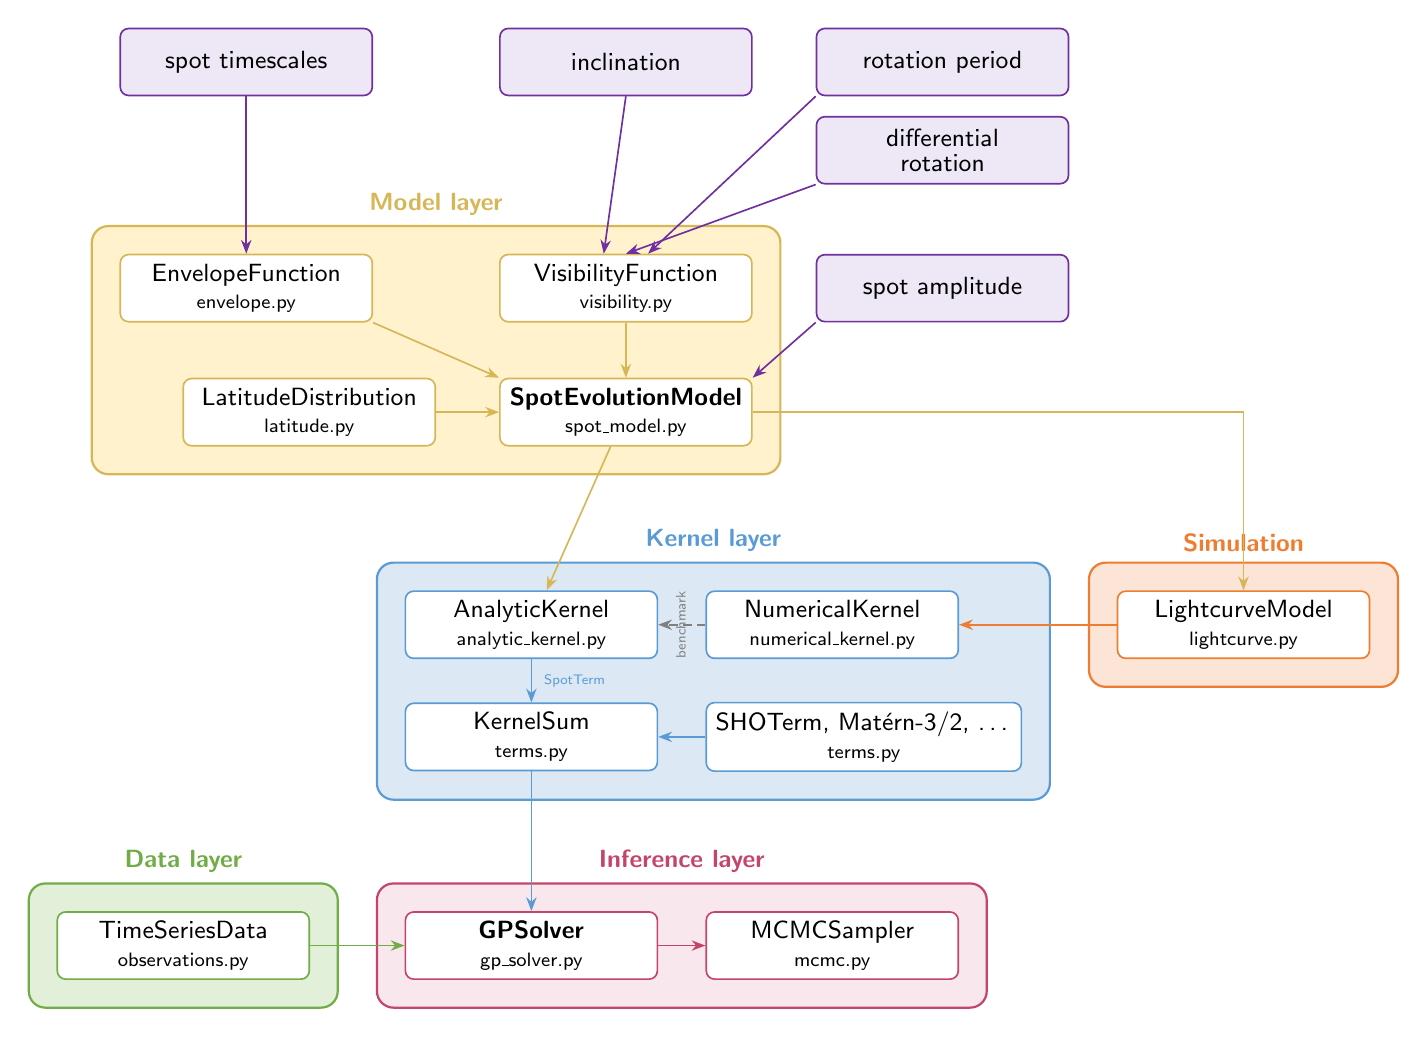
\begin{tikzpicture}[node distance=0.5cm and 0.8cm]

% ── Model layer ──────────────────────────────────────────────
% Top row: EnvelopeFunction and VisibilityFunction
\node[box=modelborder] (envbase) {EnvelopeFunction\\[-1pt]{\scriptsize envelope.py}};
\node[box=modelborder, right=1.6cm of envbase] (visbase) {VisibilityFunction\\[-1pt]{\scriptsize visibility.py}};

% Bottom row: LatitudeDistribution left of SpotEvolutionModel
\node[box=modelborder, below=0.7cm of visbase] (spotmodel) {\textbf{SpotEvolutionModel}\\[-1pt]{\scriptsize spot\_model.py}};
\node[box=modelborder, left=0.8cm of spotmodel] (latdist) {LatitudeDistribution\\[-1pt]{\scriptsize latitude.py}};

\begin{scope}[on background layer]
\node[layer={modelborder}{modelfill},
      fit=(envbase)(latdist)(visbase)(spotmodel),
      label={[layerlabel=modelborder]above:Model layer}] (mbox) {};
\end{scope}

% ── Parameter layer ──────────────────────────────────────────
% spot timescales -> EnvelopeFunction
\node[box=paramlayerborder, fill=paramlayerfill, above=2.0cm of envbase] (param_timescales) {spot timescales};

% rotation params -> VisibilityFunction
\node[box=paramlayerborder, fill=paramlayerfill] (param_inc)       at (visbase.north |- param_timescales.center) {inclination};
\node[box=paramlayerborder, fill=paramlayerfill, right=0.8cm of param_inc]      (param_rotperiod) {rotation period};
\node[box=paramlayerborder, fill=paramlayerfill, below=0.25cm of param_rotperiod] (param_diffrot) {differential\\[-2pt]rotation};

% spot amplitude -> SpotEvolutionModel (right of VisibilityFunction, same height as visbase)
\node[box=paramlayerborder, fill=paramlayerfill, right=0.8cm of visbase] (param_amp) {spot amplitude};

% Parameter arrows
\draw[arrow=paramlayerborder] (param_timescales.south) -- (envbase.north);
\draw[arrow=paramlayerborder] (param_inc.south)         -- ([xshift=-8pt]visbase.north);
\draw[arrow=paramlayerborder] (param_rotperiod.south west) -- ([xshift=8pt]visbase.north);
\draw[arrow=paramlayerborder] (param_diffrot.south west)   -- (visbase.north);
\draw[arrow=paramlayerborder] (param_amp.south west) -- (spotmodel.north east);

% Composition arrows into SpotEvolutionModel
\draw[arrow=modelborder] (envbase.south east) -- (spotmodel.north west);
\draw[arrow=modelborder] (latdist.east) -- (spotmodel.west);
\draw[arrow=modelborder] (visbase.south) -- (spotmodel.north);

% ── Inference layer (placed first to define horizontal center) ─
\node[box=infborder, below=5.9cm of spotmodel, xshift=-1.2cm] (gp) {\textbf{GPSolver}\\[-1pt]{\scriptsize gp\_solver.py}};
\node[box=infborder, right=0.6cm of gp] (mcmc) {MCMCSampler\\[-1pt]{\scriptsize mcmc.py}};

\begin{scope}[on background layer]
\node[layer={infborder}{inffill},
      fit=(gp)(mcmc),
      label={[layerlabel=infborder]above:Inference layer}] (ibox) {};
\end{scope}

% ── Data layer (left of inference, same height) ──────────────
\node[box=datalayerborder, left=1.2cm of gp] (obs) {TimeSeriesData\\[-1pt]{\scriptsize observations.py}};

% ── Kernel layer (centered above inference) ──────────────────
\node[box=kernelborder, above=3.2cm of gp] (ak) {AnalyticKernel\\[-1pt]{\scriptsize analytic\_kernel.py}};
\node[box=kernelborder, right=0.6cm of ak] (nk) {NumericalKernel\\[-1pt]{\scriptsize numerical\_kernel.py}};
\node[box=kernelborder, below=0.55cm of ak] (ksum) {KernelSum\\[-1pt]{\scriptsize terms.py}};
\node[box=kernelborder, right=0.6cm of ksum] (extraterms) {SHOTerm, Mat\'ern-3/2, \dots\\[-1pt]{\scriptsize terms.py}};

\begin{scope}[on background layer]
\node[layer={kernelborder}{kernelfill},
      fit=(ak)(nk)(ksum)(extraterms),
      label={[layerlabel=kernelborder]above:Kernel layer}] (kbox) {};
\end{scope}

% ── Simulation (same gap right of kernel as data is left of inference) ─
% Anchored off extraterms (the widest kernel-layer box) at nk's height so
% the layer boxes keep a clear gap.
\node[box=simborder, anchor=west, xshift=1.2cm] (lc) at (extraterms.east |- nk) {LightcurveModel\\[-1pt]{\scriptsize lightcurve.py}};

\begin{scope}[on background layer]
\node[layer={simborder}{simfill},
      fit=(lc),
      label={[layerlabel=simborder]above:Simulation}] (sbox) {};
\end{scope}

\begin{scope}[on background layer]
\node[layer={datalayerborder}{datalayerfill},
      fit=(obs),
      label={[layerlabel=datalayerborder]above:Data layer}] (dbox) {};
\end{scope}

% ── Cross-layer arrows ───────────────────────────────────────
\draw[arrow=datalayerborder] (obs.east) -- (gp.west);
\draw[arrow=modelborder] (spotmodel) -- (ak);
\draw[arrow=modelborder] (spotmodel.east) -| (lc.north);
\draw[arrow=kernelborder] (ak) -- node[midway, right=1pt, font=\tiny\sffamily, text=kernelborder]{SpotTerm} (ksum);
\draw[arrow=kernelborder] (extraterms.west) -- (ksum.east);
\draw[arrow=kernelborder] (ksum) -- (gp);
\draw[arrow=simborder] (lc.west) -- (nk.east);
\draw[darrow=gray] (nk.west) -- node[midway, font=\tiny\sffamily, gray, rotate=90, anchor=south, xshift=0pt, yshift=-5pt]{benchmark} (ak.east);
\draw[arrow=infborder] (gp) -- (mcmc);

\end{tikzpicture}
\end{document}
